%! TEX root = ../supernova_20yy.tex
\documentclass[../super_nova_20yy]{subfiles}

\begin{document}
\twocolumn[
  \chapter{調布祭のウラガワ $\sim$天文部が出店するまで$\sim$}

  \rightline{3年 水吉健太}
]
\small

\section{はじめに}

2024年11月22日から24日にかけて本学学園祭である「調布祭」が開催され、天文部も参加する予定です。
今年度は4月時点で新入部員42名を迎え部員数が計82名になったことや、業務用フライヤーを個人手配できる部員がいることを踏まえ、今まで行っていた教室展示に加え模擬店も出店する事となりました。
今回は、天文部が調布祭に出店するまでの様子をご紹介します。

\begin{figure}[H]
  \centering
  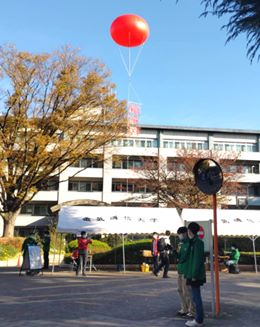
\includegraphics[width=.5\columnwidth]{画像1.jpg}
  \caption{調布祭の開催を告げる気球(2022年度調布祭)}
  \label{fig:1}
\end{figure}

\section{事前準備}

7月頃、調布祭統括係の打ち合わせで出店する食品やトッピング類を決めました。

\section{試作会}
8月頃、調布祭統括係を中心に試作会を行いました。宣材写真の背景には、実際に福島県北塩原村で撮影した天の川を印刷したものを使いました。
\begin{figure}[H]
  \centering
  \begin{minipage}[t]{0.4\columnwidth}
    \centering
    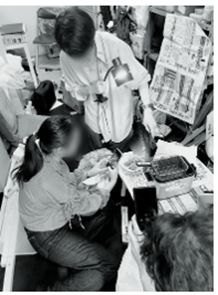
\includegraphics[width=\columnwidth]{画像2.jpg}
    \caption{宣材写真を撮影する様子}
    \label{fig:2}
  \end{minipage}
  \begin{minipage}[t]{0.4\columnwidth}
    \centering
    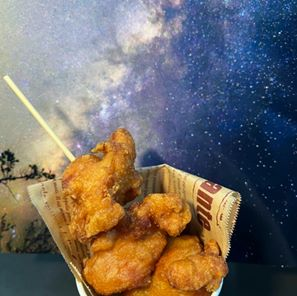
\includegraphics[width=\columnwidth]{画像3.jpg}
    \caption{完成した宣材写真}
    \label{fig:3}
  \end{minipage}
\end{figure}
\section{マスコットキャラクター}
模擬店出店に先立ち、マスコットキャラクターが誕生しました。販売促進の手助けとなってくれるはずです。

\begin{figure}[H]
  \centering
  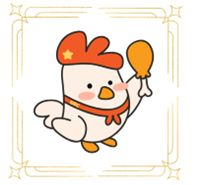
\includegraphics[width=.5\columnwidth]{画像4.jpg}
  \caption{UEC Astro チキン$_\text{くん}$}
  \label{fig:4}
\end{figure}
\section{模擬店出店場所}
天文部の出展場所は、以下の図23番との通達がありました。模擬店配置は、学友会加入率や調布祭実行委員会規定の点数等により判断されます。

\begin{figure}[H]
  \centering
  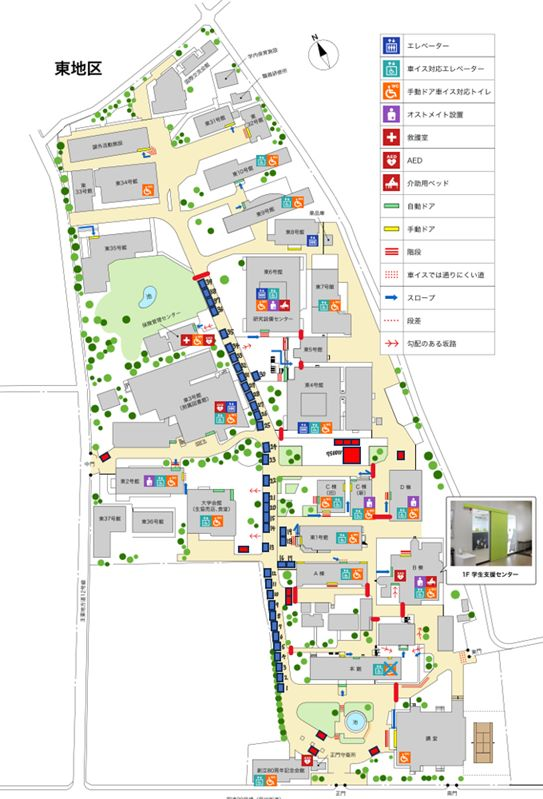
\includegraphics[width=.9\columnwidth]{画像5.jpg}
  \caption{出展場所 調布祭実行委員会第5回団体向け説明会資料より}
  \label{fig:5}
\end{figure}

\section{教室展示企画}

ここまで模擬店を紹介しましたが、教室展示の様子もご紹介します。

\section{事前準備}

調布祭統括係を中心に、係ごとに分担して準備を進めます。グッズ制作など人手が必要な作業は、係を問わず協力して作りました。
\begin{figure}[H]
  \centering
  \begin{minipage}[t]{0.4\columnwidth}
    \centering
    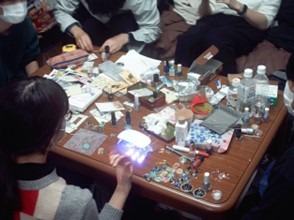
\includegraphics[width=\columnwidth]{画像6.jpg}
    \caption{グッズを作る部員}
    \label{fig:6}
  \end{minipage}
  \begin{minipage}[t]{0.4\columnwidth}
    \centering
    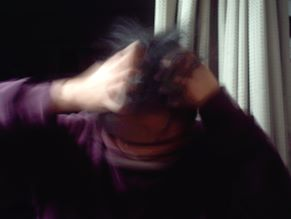
\includegraphics[width=\columnwidth]{画像7.jpg}
    \caption{部誌の締切に追われる部員}
    \label{fig:7}
  \end{minipage}
\end{figure}
\section{企画}

\begin{itemize}
  \item プラネタリウム\hbox{}\\
  天文部のメイン企画。2022年度に先代の部員が作ったものをプラネタリウム班が改良し、上映が出来るまで復元しました。また、投影機の制作や解説音声も自作しました。
  \item 天体写真展示\hbox{}\\
  部員が合宿先で撮った写真や、東3号館屋上で撮影した写真を展示します。
  \item グッズ販売\hbox{}\\
  レジンアクセサリー、缶バッチ、クリアファイル、ポストカードを用意しました。レジンは部員が一つひとつ手作りしたものです。缶バッチは、オリジナルキャラクターをもとにしたものを製作しました。\hbox{}\\
  \begin{figure}
    \centering
    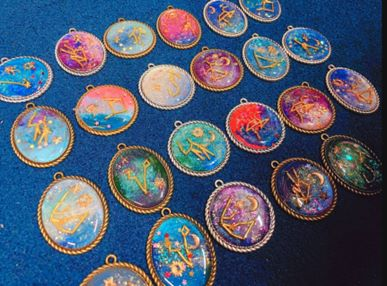
\includegraphics[width=.5\columnwidth]{画像8.jpg}
    \caption{完成したレジンキーホルダー。様々な色・形がありとても綺麗です。}
    \label{fig:8}
  \end{figure}
\end{itemize}

\section{プラネタリウム制作}

毎年調布祭で行っているプラネタリウムは、天文部のメイン企画です。昨年度の調布祭では調布祭展示大賞を頂くことが出来ました。今年はピンホール式の恒星球の制作やドームの作り変えを行い、投影できる星の数も増えています。詳しくは過去部誌「ピンホールプラネタリウム製作記」をご覧ください。

\begin{figure}[H]
  \centering
  \begin{minipage}[t]{0.4\columnwidth}
    \centering
    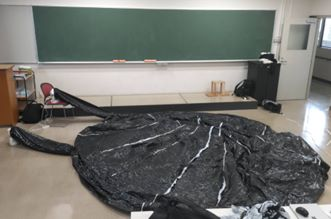
\includegraphics[width=\columnwidth]{画像9.jpg}
    \caption{膨らむ前のプラネタリウム。空気を送り込むと$\cdots$}
    \label{fig:9}
  \end{minipage}
  \begin{minipage}[t]{0.4\columnwidth}
    \centering
    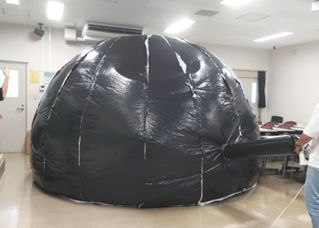
\includegraphics[width=\columnwidth]{画像10.jpg}
    \caption{空気を送り込むと天井間近まで大きくなります。この中に恒星球を入れて星や星座を投影します。}
    \label{fig:10}
  \end{minipage}
\end{figure}

\section{さいごに}
本番直前まで準備し、あとは当日を待つのみです。天文部の展示を楽しんでいただけるよう、部員一同ご来場をお待ちしております。

\onecolumn
\end{document}